\chapter{Impact de la contrainte de parcimonie sur la corpus \textit{SOUR}}\label{annexe:parcimonie}

En plus de la contrainte de régularité temporelle étudiée dans le chapitre \ref{chap:nmf_smooth}, la contrainte de parcimonie a été considérée en fin de thèse. Les résultats obtenus mériteraient donc d'être approfondis, mais les premières valeurs obtenues sont tout de même présentées dans cette annexe. Appliquée sur la matrice $\mathbf{H}$, la contrainte de parcimonie (ou \textit{sparsness}) a pour but de réduire le nombre d'éléments activés à chaque trame temporelle en pénalisant les termes non nuls. De la même façon, cette contrainte se traduit par l'ajout d'un second terme dans l'expression de la fonction de coût : 

\begin{equation}
\text{min}~D\left(\textbf{V} \Vert \textbf{WH}\right) + \alpha_{sp} C_{sp}(\mathbf{H}) \quad \text{avec} \quad \mathbf{W} \geq 0, \mathbf{H} \geq 0,
\end{equation}

avec $C_{sp}(\mathbf{H})$, la contrainte exprimée dans l'équation \ref{eq:sparsness} et $\alpha_{sp}$ la pondération. De même que pour la contrainte de \textit{smoothness}, la parcimonie est appliquée sur les matrices $\mathbf{H}$ de la NMF SUP et IS. Pour la NMF SEM, cette contrainte est appliquée non pas sur $\mathbf{H_s}$ mais sur $\mathbf{H_r}$ afin de mieux inclure des évènements ponctuels dans $\mathbf{W_r}$ et moins les composantes \textit{trafic}. La parcimonie est testée pour plusieurs valeurs de pondération : $\alpha_{sp} \in \lbrace0,05,~ 0,1,~ 0,2,~ 0,5,~ 1\rbrace$. 400 itérations sont également réalisées sur l'ensemble des combinaisons testées. Le Tableau \ref{tab:erreur_sparse} résume les erreurs $MAE_g$.

\begin{table}[h!]
\centering
\caption{Erreurs $MAE_{60}$ les plus faibles pour les combinaisons optimales des modalités des estimateurs pour le corpus d'évaluation \textit{SOUR} en présence d'une pondération de parcimonie.}
\label{tab:erreur_sparse}
\resizebox{\textwidth}{!}{%
\begin{tabular}{L{2cm}C{1.5cm}C{1.2cm}C{1.2cm}C{1.2cm}C{1.2cm}C{2.5cm}C{2.5cm}}
\toprule
\textbf{méthode} & $f_c$ (kHz) & $\beta$ & $w_t$ & $K$ & $t_h$ & $\alpha_t$ & $MAE_{60}$ \\ \toprule
\multirow{2}{*}{filtre PB} & 20 & - & - & - & - & - & 3,62 ($\pm$ 3,93) \\
 & 0,5 & - & - & - & - & - & 1,99 ($\pm$ 1,37) \\ \midrule
\multirow{4}{*}{NMF SUP}  & - & 2 & 0,5 & 25 & - & 0 & 2,13 ($\pm$ 2,22) \\ 
 & - & 0 & 0,5 & 200 & - & 0,5 & 3,73 ($\pm$ 4,01) \\
 & - & 1 & 0,5 & 50 & - & 0,05 & 2,50 ($\pm$ 1,90) \\
 & - & 2 & - & - & - & - & - \\ \midrule
\multirow{4}{*}{NMF SEM}  & - & 1 & 0,5 & 300 & - & 0 &  1,93 ($\pm$ 0,42) \\
 & - & 0 & 2 & 300 & - & 0,50 & 1,99 ($\pm$ 0,70) \\
 & - & 1 & 0,5 & 100 & - & 0,05 &  1,50 ($\pm$ 0,89) \\
 & - & 2 & - & - & - & - & - \\ \midrule
\multirow{4}{*}{NMF IS}  & - & 2 & 1 & 300 & 0,35 & 0 & 1,16 ($\pm$ 0,86) \\
 & - & 0 & \textit{all} & 50 & 0,10 & 0,44 & 1,62 ($\pm$ 1,02) \\
 & - & 1 & 1 & 200 & 0,05 & 0,40 & 1,60 ($\pm$ 0,72) \\
 & - & 2 & - & - & - & - & - \\
 \bottomrule
\end{tabular}}
\end{table}

Les résultats pour $\beta$ = 2 sur les différentes versions de la NMF ne sont pas présents en raison du comportement de la mise à jour des matrices pour ce cas. En effet, l'algorithme de mise à jour présente au numérateur une soustraction qui peut générer des valeurs négatives selon les valeurs de $\alpha_{sp}$. Ce phénomène est apparu durant les calculs et n'a pas pu être traité. Toutefois les résultats obtenus pour $\beta \in \lbrace 0,~1\rbrace$ sont correctes.
La contrainte de parcimonie a un impact différent selon la version de la NMF et les valeurs de $\beta$. Dans le cas de la NMF SUP, l'ajout de la contrainte de parcimonie n'a qu'un faible impact sur les erreurs $MAE_g$ pour la divergence KL.  Dans le cas de la NMF IS, cette contrainte ne permet pas, là encore, d'améliorer les résultats. Cette approche n'est donc pas adaptée à l'ajout de contraintes et est plus performante sans.
Une fois encore, l'influence de la contrainte est surtout notable pour la NMF SEM. Si cet impact est faible pour la divergence IS, pour la divergence KL, le gain est significatif avec une erreur $MAE_g$ de 1,50. On observe dans la Figure  \ref{fig:erreurSparseDetails} les erreurs $MAE_{60}$ pour la NMF SEM ($\beta$ = 1, $K$ = 100 et $w_t$ = 0,5 s) avec et sans pondération. On observe un comportement similaire de la méthode soumise à la parcimonie à celui obtenu avec la contrainte de régularité temporelle : une augmentation des erreurs dans \textit{Parc} pour ensuite, avec l'augmentation de la présence de trafic, diminuer de plus en plus. Cette évolution peut être illustrée, là encore, avec le spectre du signal $\mathbf{W_rH_r}$ en Figure \ref{fig:grafic_sp}. Ici c'est $\mathbf{H_r}$ qui est contraint. Dans le cas de l'ambiance \textit{Parc}, la partie libre de la NMF SEM n'est donc plus en mesure de se comporter aussi librement que sans pondération. On peut alors supposer que certains éléments \textit{trafic}, non utilisés lorsque la pondération est nulle, seront utilisés sur des sources interférantes en vue de minimiser la distance $D(\mathbf{V}\Vert \mathbf{WH})$, ce qui dégrade l'estimation du trafic.
\`A l'inverse, en présence de trafic, étant contraint d'avoir une parcimonie dans $\mathbf{H_r}$, il est moins aisé pour la NMF SEM d'y inclure des composantes \textit{trafic}, les éléments de $\mathbf{W_s}$ sont alors mieux mis à contribution que dans le cas où la pondération est nulle, ce qui permet alors d'améliorer l'estimation du signal trafic.

\begin{figure}[h]
\centering
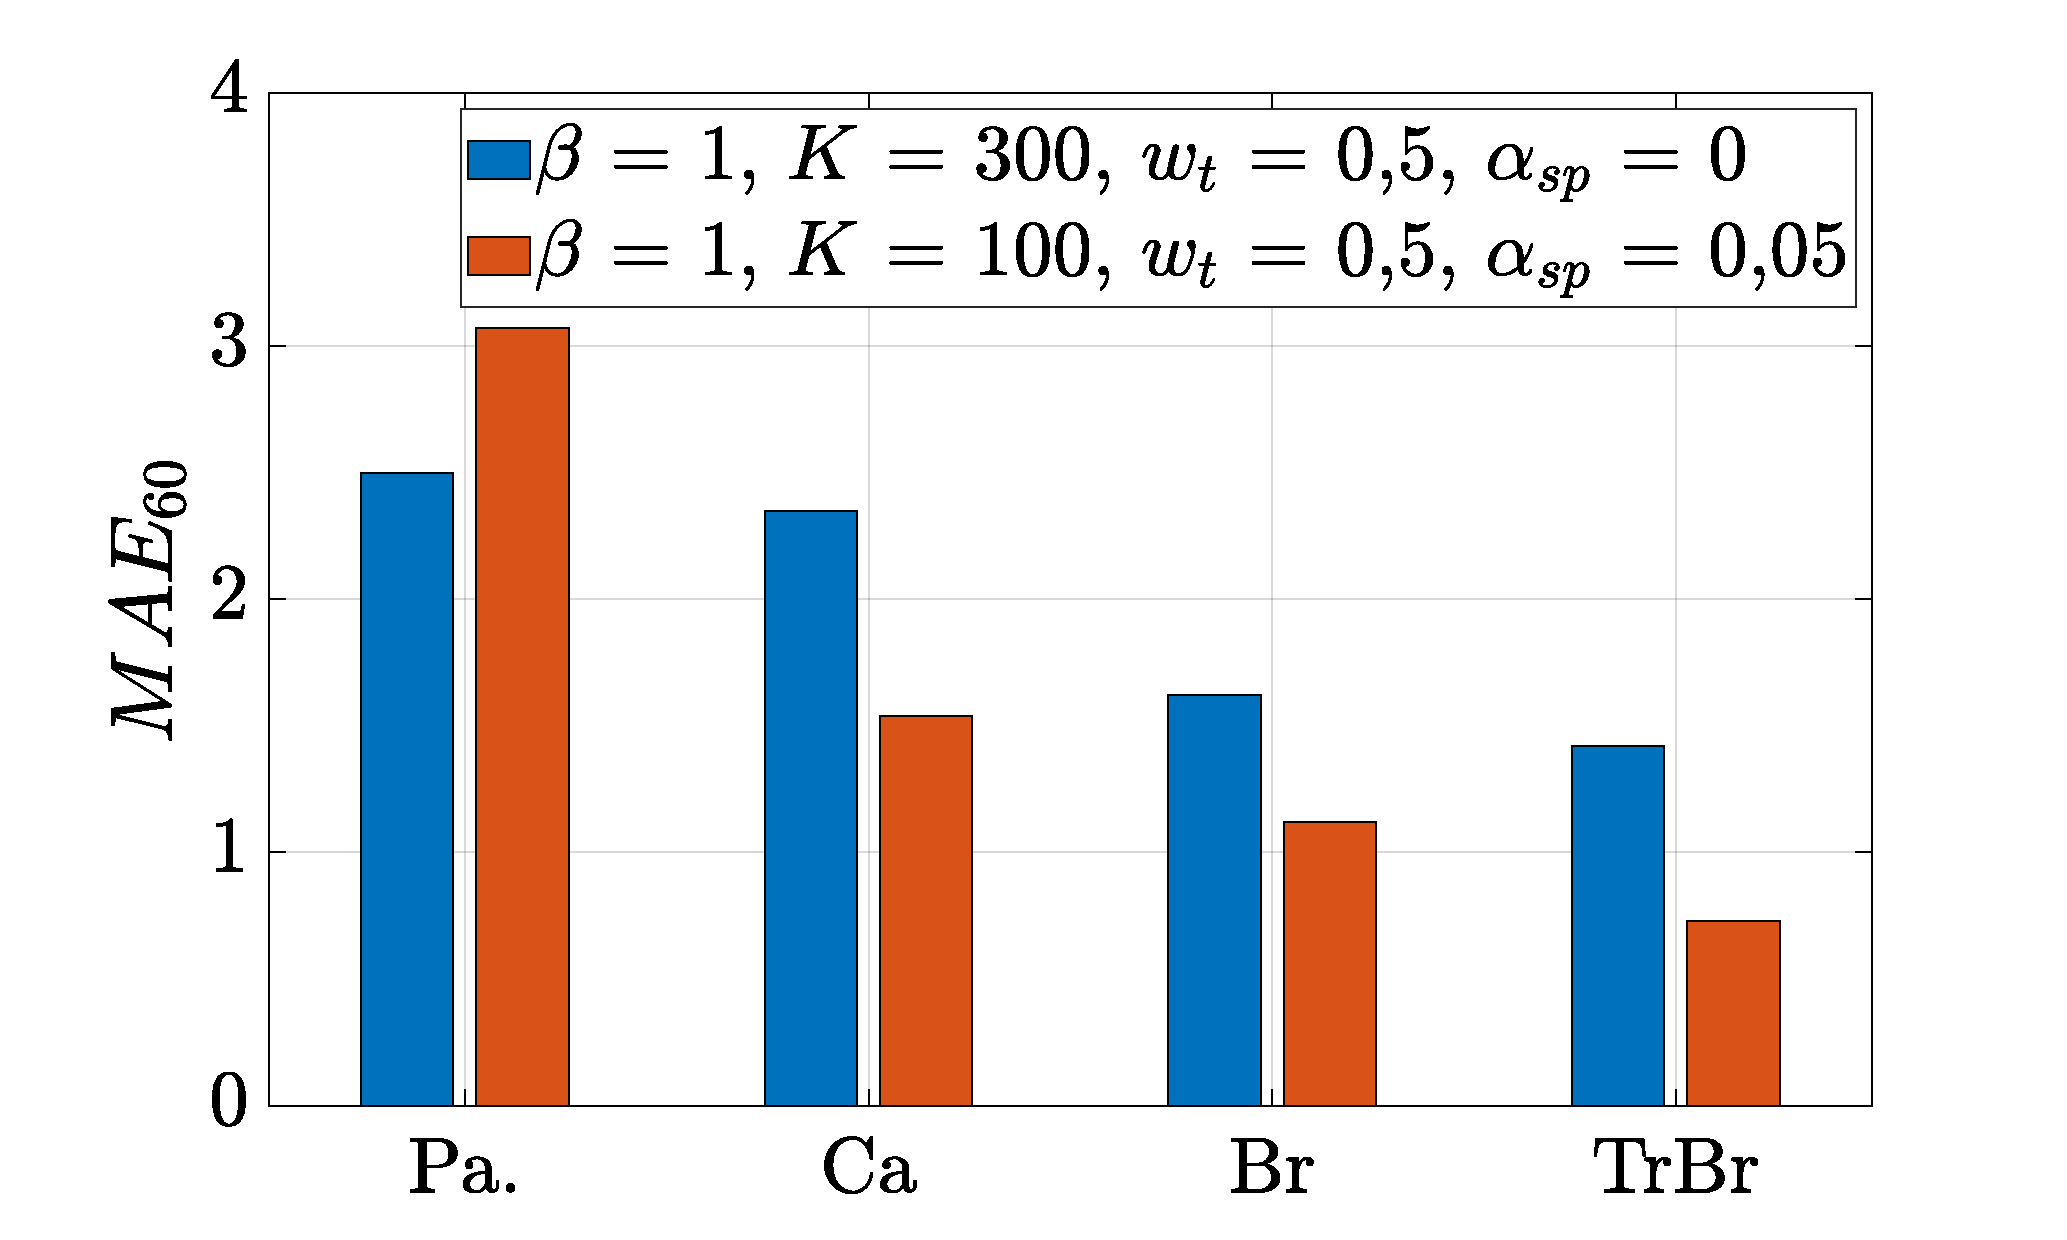
\includegraphics[width=.7\linewidth]{./figures/resultats/bar_sparse.pdf}
\caption{Influence de la parcimonie sur l'erreur $MAE_{60}$ selon la NMF SEM optimale avec et sans pondération.}
\label{fig:erreurSparseDetails}
\end{figure}

\begin{figure}[h!]
\centering
\subfigure[]{%
\label{fig:grafic_sp_park}%
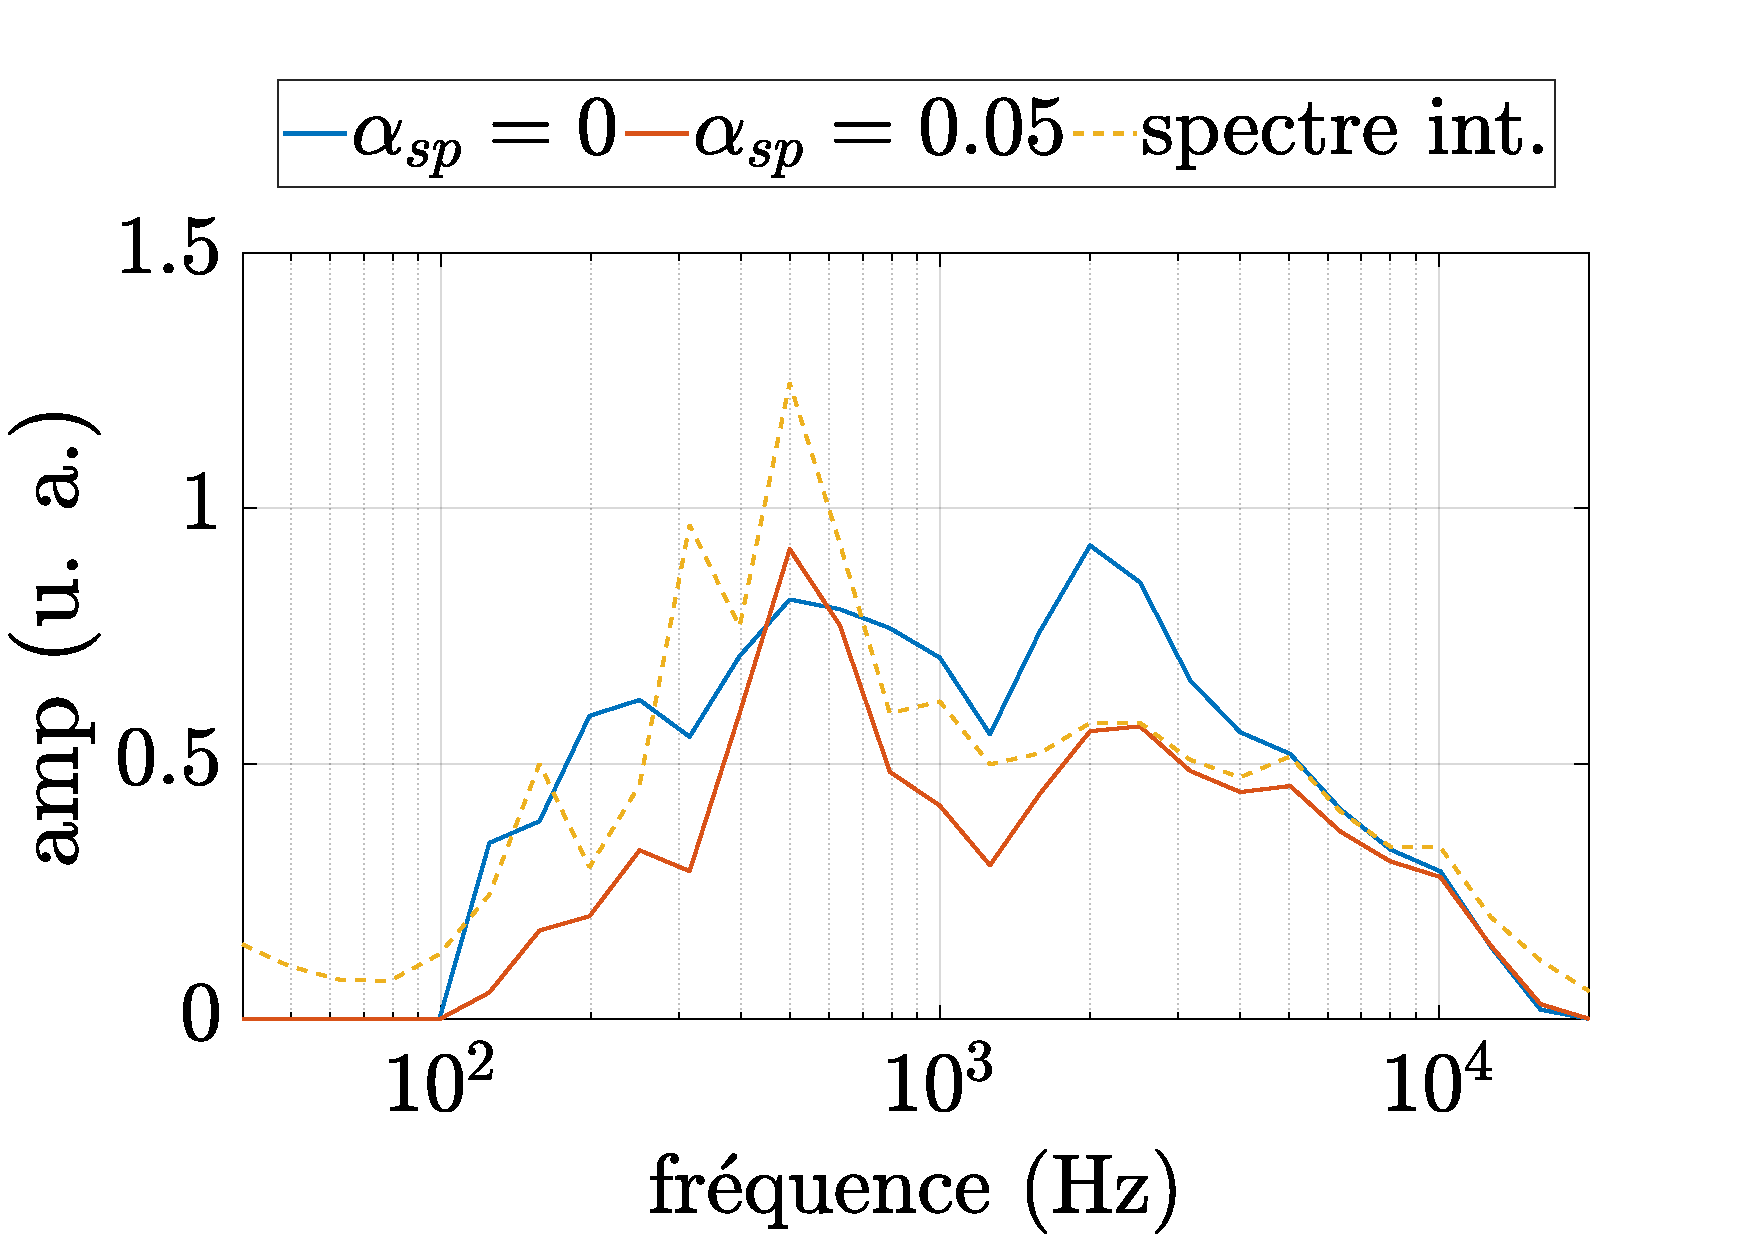
\includegraphics[width=0.45\linewidth]{./figures/resultats/example_park_SP.pdf}}%
\qquad
\subfigure[]{%
\label{fig:grafic_sp_vn}%
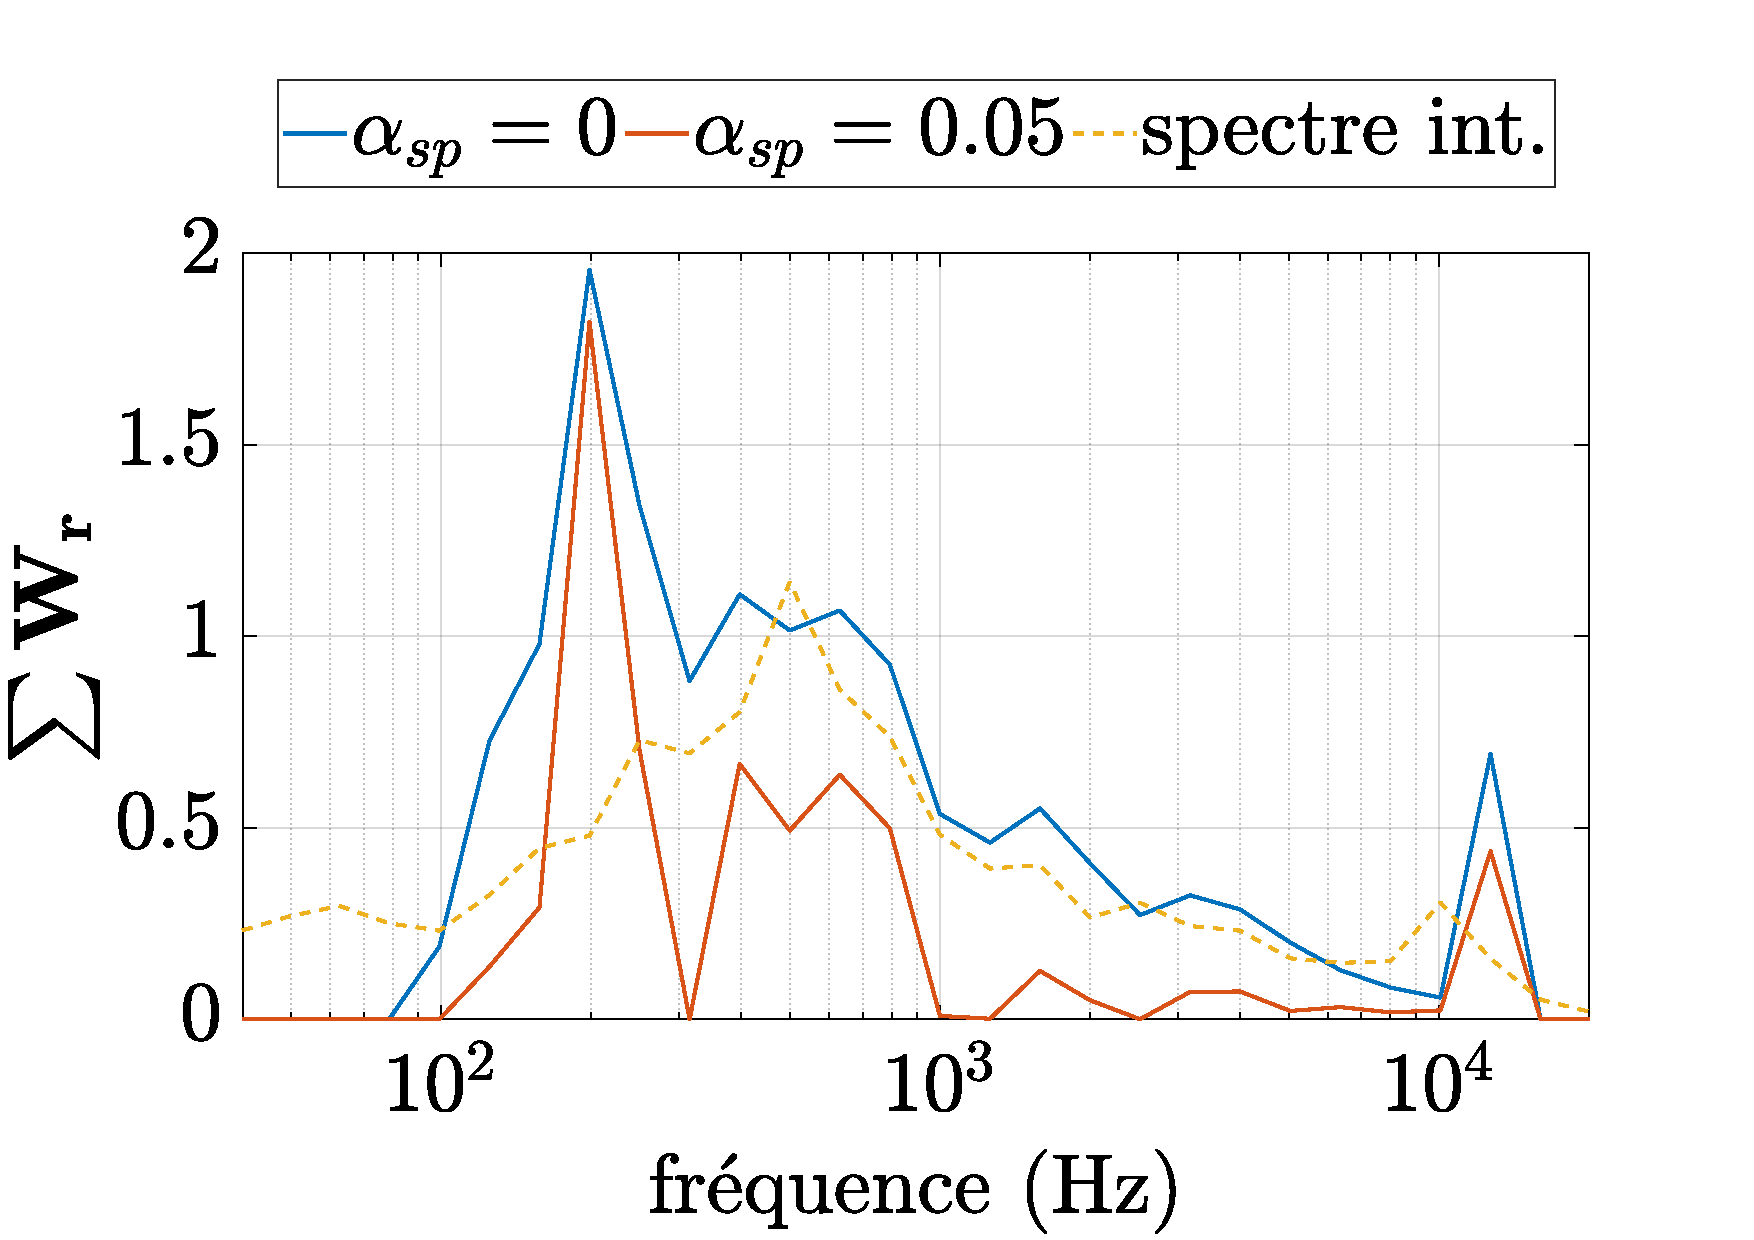
\includegraphics[width=0.45\linewidth]{./figures/resultats/example_veryNoisyStreet_SP.pdf}}%
\caption{Comparaison des spectres de la classe \textit{interférante} avec la somme des 2 éléments de $\mathbf{W_r}$ pour le cas sans pondération ($\alpha_{sp}= 0$) et avec ($\alpha_{sp} = 0,05$) pour la scène 2 de l'ambiance \textit{Parc} \subref{fig:grafic_sm_park} et la scène 7 de \textit{Rue très bruyante} \subref{fig:grafic_sm_vn}.}
\label{fig:grafic_sp}
\end{figure}

La contrainte de parcimonie a donc un impact significatif pour la NMF SEM avec $\beta$ = 1, $w_t$ = 0,5, $K$ = 100 et $\alpha_{sp}$ = 0,05. En contraignant cette fois-ci la partie libre du dictionnaire, on arrive à limiter l'ajout de composante \textit{trafic} dans la partie mobile du dictionnaire et ainsi améliorer l'estimation du niveau sonore du trafic. Cette contrainte engendre toutefois une augmentation des erreurs dans l'ambiance \textit{Parc}. Son impact sur la NMF IS reste, comme la contrainte de régularité temporelle, négatif et dégrade les estimation du niveau sonore du trafic.